\hypertarget{ux642dux5efaux5f00ux53d1ux73afux5883}{%
\subsection{搭建开发环境}\label{ux642dux5efaux5f00ux53d1ux73afux5883}}

使用 MicroPython
开发机器人,我们首先要搭建一个开发环境。和运行在桌面或服务器的纯软件环境不同的是,我们得有一个硬件开发环境。可以选择树莓派
+ Arduino
控制板,但是搭建机器人需要的零件比较复杂。作为教程,我们选择乐高 EV3
机器人作为开发环境,因为乐高机器人搭建非常容易,并且乐高的 EV3
控制器是一个完整的 ARM 系统。

那么问题来了:如果你没有乐高 EV3 怎么办?

戳这里:EV3 教育版淘宝\href{https://s.click.taobao.com/PeMmziv}{链接
1}、\href{https://s.click.taobao.com/VsKmziv}{链接 2},EV3
零售版淘宝\href{https://s.click.taobao.com/UMLmziv}{链接
1}、\href{https://s.click.taobao.com/PuMmziv}{链接 2}。教育版建议买
45544+45560 套装,零售版就只有 31313 一种。没有 MicroSD
卡的可以顺手入一个 MicroSD 卡 +
读卡器,还可以再选购一个蓝牙游戏手柄,后面用得到。

乐高官方提供了一个完整的 EV3 运行时镜像,该镜像内置了
MicroPython,可以非常方便地运行 Python
程序。需要从乐高官网\href{https://education.lego.com/en-us/support/mindstorms-ev3/python-for-ev3}{下载镜像}到本地,然后写入到
MicroSD 卡。Windows 和 Mac 系统可以使用
\href{https://www.balena.io/etcher/}{Etcher} 写入镜像到 MicroSD
卡,也可以使用\texttt{dd}命令写入。

插入 SD 卡后启动 EV3 控制器,等待 1\textasciitilde2
分钟,启动成功后,即可选择 ``Wireless and Networks'' 连接电脑:

 
 \begin{figure}[htp]
	\centering
	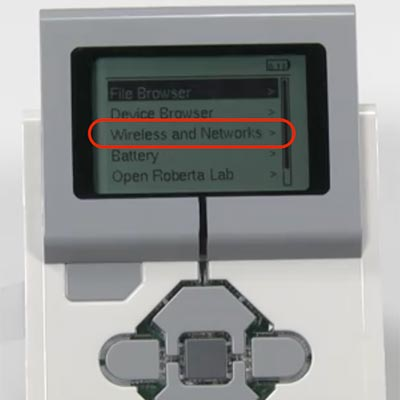
\includegraphics[width=0.6\linewidth]{fig/1346188160794690l.png}
\end{figure}


使用无线网连接需要额外的 USB 无线网卡,强烈推荐选择蓝牙连接,因为 EV3
内置了蓝牙模块。配对并连接成功后,可以在电脑上看到已连接的蓝牙设备 EV3。

可以直接使用 SSH 登录 EV3,因为这个自带 MicroPython 的 EV3
镜像是一个裁剪后的 Debian Linux
系统。我们用命令\texttt{ssh\ robot@ev3dev.local}登录,密码是\texttt{maker}:

\begin{pythoncode}
$ ssh robot@ev3dev.local
Password: *****
Linux ev3dev 4.14.96-ev3dev-2.3.2-ev3 
             _____     _
   _____   _|___ /  __| | _____   __
  / _ \ \ / / |_ \ / _` |/ _ \ \ / /
 |  __/\ V / ___) | (_| |  __/\ V /
  \___| \_/ |____/ \__,_|\___| \_/

Debian stretch on LEGO MINDSTORMS EV3!
Last login: Mon Mar  4 18:05:04 2019 from f81e::a7:c54d:4e0b:3af7%bnep0
robot@ev3dev:~$ ls /usr/lib/micropython/
README           fcntl.mpy      mailbox.mpy          reprlib.mpy       trace.mpy
README.rst       ffilib.mpy     mailcap.mpy          runpy.mpy         traceback.mpy
__future__.mpy   fnmatch.mpy    mimetypes.mpy        sched.mpy         tty.mpy
_libc.mpy        formatter.mpy  multiprocessing.mpy  sdist_upip.mpy    types.mpy
_markupbase.mpy  fractions.mpy  nntplib.mpy          select.mpy        typing.mpy
abc.mpy          ftplib.mpy     numbers.mpy          selectors.mpy     uaiohttpclient.mpy
argparse.mpy     functools.mpy  operator.mpy         shelve.mpy        uasyncio
base64.mpy       getopt.mpy     optparse.mpy         shlex.mpy         uasyncio.mpy
binascii.mpy     getpass.mpy    os                   shutil.mpy        ucontextlib.mpy
binhex.mpy       gettext.mpy    pathlib.mpy          signal.mpy        ucurses
bisect.mpy       glob.mpy       pdb.mpy              smtplib.mpy       udnspkt.mpy
calendar.mpy     gzip.mpy       pickle.mpy           socket.mpy        umqtt
cgi.mpy          hashlib        pickletools.mpy      socketserver.mpy  unicodedata.mpy
cmd.mpy          heapq.mpy      pkg_resources.mpy    sqlite3.mpy       unittest.mpy
code.mpy         hmac.mpy       pkgutil.mpy          ssl.mpy           upip.mpy
codecs.mpy       html           platform.mpy         stat.mpy          upip_utarfile.mpy
codeop.mpy       http           poplib.mpy           statistics.mpy    upysh.mpy
collections      imaplib.mpy    posixpath.mpy        string.mpy        urequests.mpy
concurrent       imp.mpy        pprint.mpy           stringprep.mpy    urllib
contextlib.mpy   importlib.mpy  profile.mpy          struct.mpy        urllib.mpy
copy.mpy         inspect.mpy    pty.mpy              subprocess.mpy    utarfile.mpy
csv.mpy          io.mpy         pwd.mpy              sys.mpy           uu.mpy
curses           ipaddress.mpy  pyb.mpy              tarfile.mpy       uuid.mpy
datetime.mpy     itertools.mpy  pystone.mpy          telnetlib.mpy     venv.mpy
dbm.mpy          json           pystone_lowmem.mpy   tempfile.mpy      warnings.mpy
decimal.mpy      keyword.mpy    queue.mpy            test              weakref.mpy
difflib.mpy      linecache.mpy  quopri.mpy           textwrap.mpy      xmltok.mpy
email            locale.mpy     random.mpy           threading.mpy     zipfile.mpy
errno.mpy        logging.mpy    re.mpy               time.mpy          zlib.mpy
ev3dev2          machine        readline.mpy         timeit.mpy
\end{pythoncode}

在\texttt{/usr/lib/micropython/}目录下可以看到系统自带的 Python
库。MicroPython
并不直接运行\texttt{.py}文件,而是运行\texttt{.mpy}这个紧凑的二进制文件。

要开发 EV3 机器人程序,我们还需要搭建一个开发环境。Visual Studio Code
是强烈推荐的开发环境,并且,乐高官方推出了一个 VSCode
扩展,可以方便地开发并远程调试应用程序。在 VS Code
的扩展中搜索\texttt{lego}并安装\texttt{LEGO®\ MINDSTORMS®\ EV3\ MicroPython}扩展:

 
 \begin{figure}[htp]
	\centering
	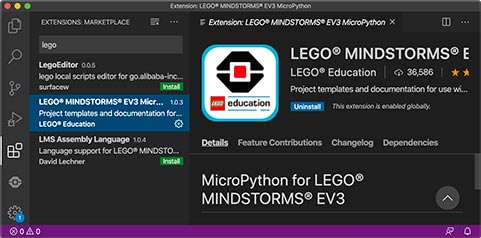
\includegraphics[width=0.6\linewidth]{fig/1346189421183041l.png}
\end{figure}


安装扩展后,我们就可以开始开发运行在 EV3 上的 Python 程序。在 VS Code
左侧面板选择 Lego 图标,选择 ``Create a new project'':

 
 \begin{figure}[htp]
	\centering
	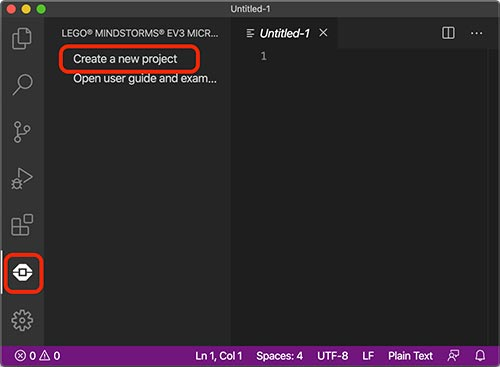
\includegraphics[width=0.6\linewidth]{fig/1346190218100802l.png}
\end{figure}


我们创建一个\texttt{hellorobot}的工程,EV3
插件自动为我们创建了一个包含样板代码的\texttt{main.py}:

\begin{pythoncode}
from pybricks import ev3brick as brick
from pybricks.ev3devices import (Motor, TouchSensor, ColorSensor, InfraredSensor, UltrasonicSensor, GyroSensor)
from pybricks.parameters import (Port, Stop, Direction, Button, Color, SoundFile, ImageFile, Align)
from pybricks.tools import print, wait, StopWatch
from pybricks.robotics import DriveBase
brick.sound.beep()
\end{pythoncode}

首行的注释表示运行环境是 MicroPython,然后自动导入了 EV3 所需的所有控制
API。\texttt{brick.sound.beep()}用于控制 EV3 的扬声器发出一声 ``哔''
的声音。

我们可以编写任意的 Python
源码文件,但执行时注意程序入口永远是\texttt{main.py}。

在 VS Code
中,找到\texttt{EV3DEV\ DEVICE\ BROWSER},点击\texttt{ev3dev},连接后图标显示为绿色:

 
 \begin{figure}[htp]
	\centering
	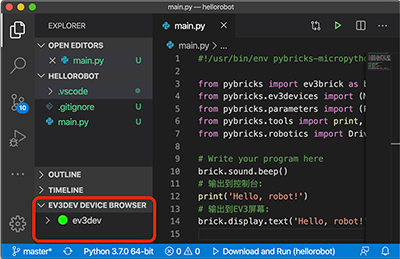
\includegraphics[width=0.6\linewidth]{fig/1346267955331105l.png}
\end{figure}


接下来,我们就可以直接切换到 Run
面板,点击\texttt{RUN}运行,在\texttt{OUTPUT}面板中看到输出结果:

 
 \begin{figure}[htp]
	\centering
	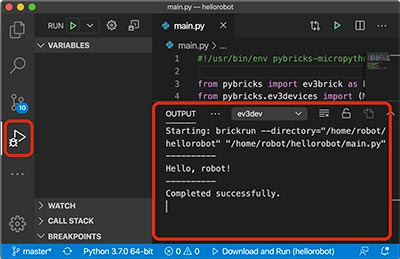
\includegraphics[width=0.6\linewidth]{fig/1346268110520386l.png}
\end{figure}


注意到 VS Code 是一个开发环境,我们在电脑上并没有安装
MicroPython,整个程序是通过蓝牙网络先传输到 EV3
主机,再执行,最后取回输出结果显示在 VS Code
中,因此,这是一个远程执行并允许调试的功能。\texttt{print()}函数可以输出到
VS Code,主要作为调试使用,\texttt{brick.display.text()}则是输出到 EV3
的主机屏幕上。

这样,我们就把连接 EV3 的整个 MicroPython 开发环境搭建好了。

\hypertarget{ux53c2ux8003ux6e90ux7801}{%
\subsubsection{参考源码}\label{ux53c2ux8003ux6e90ux7801}}

\href{https://github.com/michaelliao/learn-python3/tree/master/samples/micropython/hellorobot}{hellorobot}

